\chapter{Pregled korištenih tehnologija}

\section{NFC \textit{(en. near-field communication)}}
NFC skup komunikacijskih protokola omogućava uspostavu komunikacijskog kanala između dva uređaja koji se nalaze u neposrednoj blizini jedan drugog (1-4 cm) i razmjenu podataka između njih\cite{NFCProtocol}. Komunikacija se odvija na način da MASTER uređaj osluškuje signal na prijemniku i u slučaju detektovanje SLAVE signala uređaja pošiljaoca, propisanog istim standardom zaprima podatke i vrši obradu nad njima, komunikacija se u većini slučajeva odvija jednosmjerno kratkim standardiziranim porukama (NDEF), no moguće je ostvariti i half-duplex komunikaciju između uređaja, kao i razmjenu nestandardnih poruka, u kojem slučaju se sam korisnik mora pobrinuti za implementaciju kompletnog komunikacijskog protokola. Potpuni detalji implementacija dati su u referencama relevantnih standarda u nastavku tehničkog pregleda, odličnu sintezu detalja i implementacije daju Igoe, Coleman i Jepson\cite{Igoe2014}.
\subsection{NXP NTAG216}
U cilju zadovoljenja postavljenih funkcionalnih zahtjeva bilo je neophodno odabrati NFC Tag platformu koja će odrediti relevantne standarde pohrane binarnih podataka na uređajima kao i pripadajuće komunikacijske protokole, također dodatno su postavljeni zahtjevi ekonomičnosti implementacije i kompatibilnosti sa postojećim čitačima. Uzimajući u obzir nabrojane kriterije odabrana je platforma NTAG216 proizvođača NXP Semiconductors\cite{NTAG216} bazirana na NFC Forum Tag tipu 2 i ISO/IEC14443 Tip A specifikaciji\cite{NFCTag2}\cite{ISO14443}. 

\paragraph*{}
Mogućnosti navedene platforme dostatne su za ispunjenje navedenih funkcionalnih uslova, a pružaju i neke dodatne sigurnosne mehanizme - poput neizmjenjivog jedinstvenog serijskog broja svakog taga (Tag UID) potpisanog kriptografskim ključem proizvođača, navedena funkcionalnost nije implementirana u predstavljenom rješenju jer se bazira na zaštićenoj NXP tehnologiji i nije kompatibilna sa HCE emulacijom, no umnogome može doprinijeti ukupnoj sigurnosti fizičkih Tag čipova u slučaju produkcijske implementacije rješenja. U nastavku je data proizvođačka lista izdvojenih funkcionalnosti NTAG216:

\begin{itemize}[noitemsep]
    \item 7-bajtni UID programiran od strane proizvođača za svaki tag
    \item mogućnost jednokratnog programiranja i zaključavanja taga za dalje izmjene
    \item mogućnost read-only zaključavanja taga
    \item potpis originalnosti baziran na kriptografiji eliptičnih krivih
    \item zaštita memorijskih operacija 32-bitnom lozinkom
\end{itemize}

\begin{figure}[H]
    \centering
    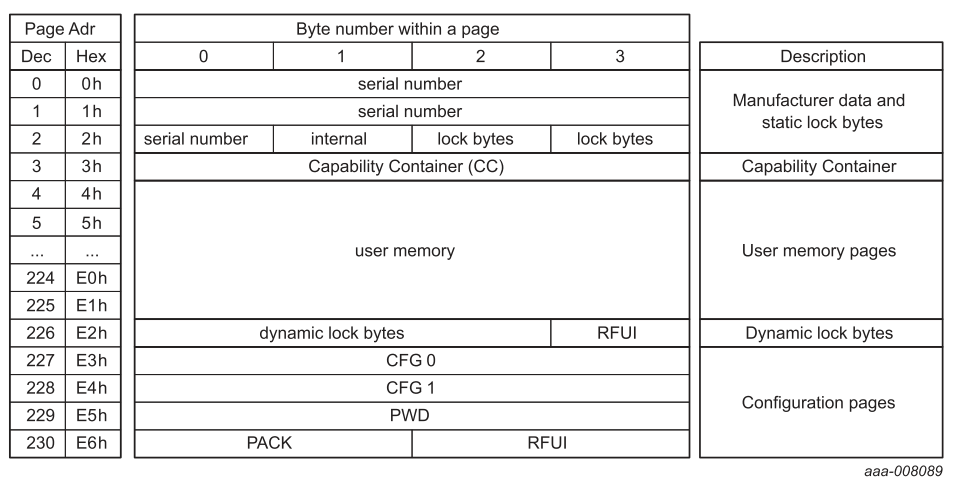
\includegraphics[width=1\textwidth]{material/ntag216-memory}
    \caption{NTAG216 organizacija memorije\cite{NTAG216}}
\end{figure}

\subsection{NDEF \textit{(en. NFC Data Exchange Format)}}
NDEF specifikacija definiše \textbf{format enkapsulacije poruke} za razmjenu informacija između dva NFC uređaja. NDEF je lagan binarni format poruke i može se koristiti za enkapsulaciju jednog ili više aplikacijski-definisanih tereta \textit{(en. payload)} raznih vrsta i veličina unutar jedne NDEF poruke. Svaki teret opisan je od strane tipa, dužine i opcionalnog identifikatora. Identifikatori tipa mogu biti URI, MIME media tipovi, ili NFC-specifični tipovi. NDEF je striktno \textbf{format} poruke i ne poznaje pojam konekcije ili logičkog kola.\cite{NDEF}

\paragraph*{}
Neki od ciljeva koje NDEF nastoji da ispuni:
\begin{itemize}[noitemsep]
    \item enkapsulacija dokumenata i binarnih objekata, slika etc.
    \item enkapsulacija podataka nepoznate dužine, npr. stream-a podataka
    \item agregacija srodnih sadržaja unutar jedne poruke
    \item kompaktna enkapsulacija malih datagrama
\end{itemize}

\subsection{HCE \textit{(en. Host card emulation)}}
HCE je metod emuliranja virtuelnog identifikacijskog modula korisnika, u osnovi to je način zaobilaska hardverskih ograničenja (\textit{en. hack, workaround}) koja onemogućavaju direktan pristup SIM (\textit{en. Subscriber Identification Module}) modulu kod mobilnih telefonskih uređaja\cite{elenkov_2012}, ovakvo rješenje vuće korijene iz ekonomske realnosti sektora mobilnih komunikacija i kartičnog plaćanja, koja se najpreciznije može okarakterisati kao oligopol, naime Google je nastojao integrisati SIM karticu unutar Android operativnog sistema u vidu eSE (\textit{en. embedded Secure Element}) korištenjem već postojeće SIM kartice operatera a u svrhu razvoja Google Wallet rješenja, no to nije odgovaralo operaterima i odbili su suradnju, nakon toga Google iznalazi alternativne načine rješenja problema poput HCE\cite{randomoracle_2014}.

\begin{figure}[H]
    \centering
    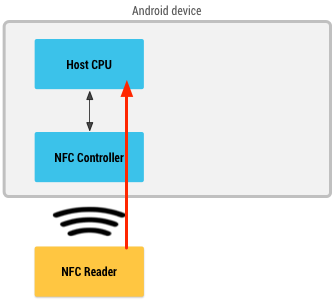
\includegraphics[width=0.6\textwidth]{material/host-based-card}
    \caption{NFC HCE virtuelnog sigurnog elementa (SE)\cite{androidhce_2018}}
\end{figure}

\paragraph*{}
HCE na Android OS radi, kako i naziv govori u CE (\textit{en. Card Emulation}) SLAVE modu, gdje se na svaki BUMP sa NFC čitačem odašilju pripremljeni podaci. Podaci koji se pri tome šalju moraju pratiti standard kartice koju žele emulirati i najčešće se vrši prijenos dokumenta ili datagrama unutar jednog ili više NDEF paketa. Logit koristi pristup prijenosa JSON formatiranog SPIM objekta \texttt{plain/text} unutar jednog NDEF paketa. Radi se o konceptu sa mnoštvom implementacijskih detalja, te zbog sažetosti za više detalja konsultujte oficijelnu dokumentaciju \url{https://developer.android.com/guide/topics/connectivity/nfc/hce}, dok je izvrstan logički prikaz sa primjerima dao Elenkov\cite{Elenkov2015}.

%(\textit{en. })
%https://developer.android.com/guide/topics/connectivity/nfc/hce
%ttps://nelenkov.blogspot.com/2012/08/accessing-embedded-secure-element-in.html
%https://nelenkov.blogspot.com/2012/08/android-secure-element-execution.html
%https://nelenkov.blogspot.com/2012/08/exploring-google-wallet-using-secure.html
%UICCs are actually smart cards that can host applications, and as such are one form of a SE. However, since the UICC is only connected to the basedband processor, which is separate from the application processor that runs the main device OS, they cannot be accessed directly from Android. All communication needs to go through the Radio Interface Layer (RIL) which is essentially a proprietary IPC interface to the baseband. 
%there is currently no standard way to communicate with the UICC SE through the RIL
%
%The Single Wire Protocol (SWP) is a specification for a single-wire connection between the SIM card and a near field communication (NFC) chip in a cell phone. It is currently under final review by the European Telecommunications Standards Institute (ETSI).[1][2]
% ETSI TS 102 613 V.11.0.0 - UICC-CLF Interface; Part 1: Physical and data link layer characteristics (Release 11)
%  ETSI TS 102 622 V.12.1.0 - UICC-CLF Interface; Host Controller Interface (HCI) (Release 12)
%  https://en.wikipedia.org/wiki/Single_Wire_Protocol
%This is the case in the Nexus S, as well as the Galaxy Nexus, and while this functionality is supported by the NFC controller drivers, it is disabled by default.
%
%NFC and the SE are tightly integrated in Android, and not only because they share the same silicon, so let's say a few words about NFC. NFC has three standard modes of operation: 
%reader/writer (R/W) mode, allowing for accessing external NFC tags 
%peer-to-peer (P2P) mode, allowing for data exchange between two NFC devices (Android Beam)
%card emulation (CE) mode, which allows the device to emulate a traditional contactless smart card 
%
%https://randomoracle.wordpress.com/2014/08/12/fakeid-android-nfc-stack-and-google-wallet-part-i/
%
%https://randomoracle.wordpress.com/2013/12/02/nfc-card-emulation-and-android-4-4-part-i/
%
%HCE je inicijalno bio direktno nakacen na eSE, kasnije je i i sam Google presao na host emulaciju, razlog za ugradnju SE cipa je bio jer telekom operateri nisu dopustili Googlu pristup njihovom SE, naknadno je google kupio taj njihov projekat ISIS, koji je izgleda na kraju i napusten.
%
%Turning the screen on enables card-emulation mode on Android devices by default. (Note it is not necessary to unlock the screen, similar to how payments can be executed by tapping the point-of-sale terminal.)
%When the phone is introduced to the NFC field of the smartcard reader in this state, Windows smart-card service registers it as a card-present event.
%Appearance of a new card triggers a discovery process, to determine what type of card the user has introduced. End goal is picking a suitable smart-card driver. Because applications using smart-card operate in terms of higher level of abstractions such as certificates and cryptographic keys, drivers are required to translate these into low-level commands that each type of card understands.
%During the discovery process, the PC will exchange traffic over NFC with the secure element, to query its features.
%Driver discovery fails. This is not surprising– the “card” in question is used for contactless payments. It does not implement any of the standard card edges built into Windows 7/8 (PIV and GIDS) and neither does the answer-to-reset (ATR) identifier returned by the secure element
%Because no driver is located, the higher level application– in this case Windows logon– also fails in its attempt to locate credentials on the card, displaying the error in the last screenshot.
%https://randomoracle.wordpress.com/2012/11/25/your-android-phone-is-also-a-smartcard/
%
%The first post in this series described the permissions model for accessing the Android secure element from its contact interface. (Not to be confused with access from contactless aka NFC interface, which is open to any external device in NFC range.) This model can be viewed as a generalization of standard Android signature-based permissions— in fact for Gingerbread it was a vanilla signature permission based on matching the certificate used for signing NFC service.
%
%Starting with ICS, there is an explicit whitelist of allowed signing certificates. Any user application signed with one of these keys can obtain access to the secure element, and more broadly to administrative actions involving the NFC controller such as toggling card emulation mode.
%https://randomoracle.wordpress.com/2013/01/19/using-the-secure-element-on-an-android-device-23/
\section{Ostalo}
Dodatno koristi se Android arhitektura za dobaljanje geolokacije\cite{geoa} uz reverzno geokodiranje od strane OpenStreetMap Nominatim projekta\cite{nominatim}. Za potpisivanje i enkripciju korisničkih podataka koristi se RSA\cite{rivest1978method} kriptografija sa 2048 bit ključem. LAPI je Python flask API i koristi UPnP, kompletan listing koda prikazan je u dodatku.